\section{Study A: Selective Branch Adaptation}
\label{sec:paired-results}

\begin{table}[t]
\centering\small
\setlength{\tabcolsep}{5pt}
% GENERATED by evidence/build_manuscript_numbers.py
\begin{tabular}{lrrrrrrr}
\toprule
Method & Prec. & Recall & $F_1$ & Exact & Pred./Gold & Spurious & Missed \\
\midrule
Direct & 0.481 & 0.758 & 0.588 & 0.333 & 52/33 & 27 & 8 \\
Graph as context & 0.431 & 0.939 & 0.590 & 0.148 & 72/33 & 41 & 2 \\
Evidence-first & 0.235 & 0.485 & 0.317 & 0.074 & 68/33 & 52 & 17 \\
\casepath & \textbf{0.615} & 0.727 & \textbf{0.667} & \textbf{0.444} & 39/33 & \textbf{15} & 9 \\
\bottomrule
\end{tabular}

\caption{\textbf{Held-out signed-change evaluation} (\nPairsHid{} pairs,
\nGoldAtoms{} reference changes). Correct, spurious and missed count signed changes. Exact counts pairs
whose entire signed set is reproduced; $F_1$ includes its 95\%
family-cluster bootstrap interval. These are errors in changes between two checklists, not
requests in a complete claim.}
\label{tab:main}
\end{table}



\paragraph{Fewer unjustified changes.}
Table~\ref{tab:main} reports the held-out comparison. \casepath predicts \cpPred{} signed changes for \nGoldAtoms{}
reference changes: \cpTP{} correct, \cpSpur{} spurious, \cpMiss{} missed.
Direct predicts \dirPred{} (\dirTP{} correct, \dirSpur{} spurious), Graph as
context \gcPred{} (\gcTP, \gcSpur) and Evidence-first \efPred{} (\efTP,
\efSpur). \casepath thus makes \redDir\%, \redGc\% and \redEf\% fewer
spurious changes than the three alternatives while keeping recall \cpRec,
and it reproduces the whole signed set on \cpExactN{} of \nPairsHid{} pairs
against \dirExactN, \gcExactN{} and \efExactN. Graph as context recovers the
most reference changes (\gcTP{} of \nGoldAtoms) at the cost of \gcSpur{}
spurious ones. In this comparison, providing the graph as context improves
recall but does not impose the controller's restriction on what may be requested. The contrast with Direct is precise:
twelve fewer false-positive changes for one fewer correct change.

A retrospective partition sharpens the interpretation: \eoCpOutside{} of
\casepath's \cpSpur{} spurious changes concern documents outside the
benchmark's branch-governed set, compared with all \eoDirOutside,
\eoGcOutside{} and \eoEfOutside{} comparator errors. Process control reduces
this form of checklist drift; it does not eliminate it. The partition does
not identify universally required baseline documents, which the signed-change
references do not specify.

\paragraph{How much does the result generalize?}
Family-cluster intervals are wide: $F_1$ \cpF{} $[\cpCIlo,\cpCIhi]$ for
\casepath against $[\dirCIlo,\dirCIhi]$ and $[\gcCIlo,\gcCIhi]$ for the two
strongest comparators, with paired differences $[\dDirLo,\dDirHi]$ and
$[\dGcLo,\dGcHi]$ that include zero; only the contrast with Evidence-first
excludes it ($[\dEfLo,\dEfHi]$). The broad-superiority gate fails on three
of its eight conditions (Table~\ref{tab:gates}): margins \mDir{} and \mGc{}
fall short of $\gateMargin$, precision \cpPrec{} falls short of $\gatePrec$, and the
Holm-adjusted family-swap $p$-values are \pHolmDir, \pHolmGc{} and \pHolmEf.
The count reduction supports selectivity on these pairs; the preregistered
criterion for broad superiority is not met.

\paragraph{Branch specificity.}
Holding \casepath's outputs fixed and pairing them with the wrong branch
families collapses signed-change $F_1$ from \wpObs{} to a maximum of
\wpMax{} over the \wpEvaluated{} evaluated reassignments (mean \wpMean;
add-one randomisation $p=\wpP$). The changes are specific to the intervened
branch. This does not identify the internal representation as the only
possible cause; a family-specific lookup would also pass. Two structural
facts are separate from accuracy: all \chainAttributed{} of \chainPredicted{}
predicted changes are attributed in the retained records to a changed guard,
including the incorrect ones, and \chainCovered{} of \nGoldAtoms{} reference
changes (\chainCoverage\%) are reachable through a source chain in the frozen
representation. Attribution is an invariant of the architecture, not evidence
that a mapping was right; reachability says a route existed, not that it was
emitted.

\begin{figure}[t]
\centering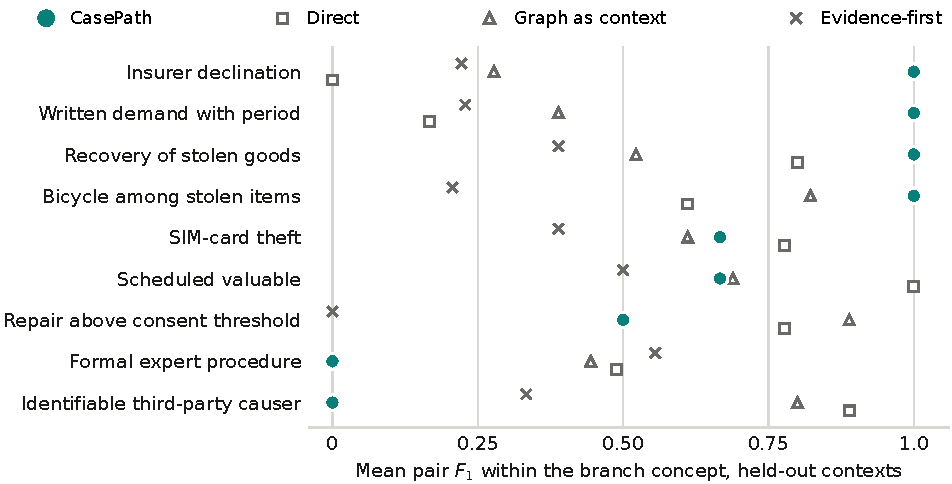
\includegraphics[width=\linewidth]{fig_family_results.pdf}
\caption{\textbf{Where the semantics holds and where it fails.} Mean pair
$F_1$ per branch concept on the held-out contexts: the marker is \casepath,
the square, triangle and cross identify Direct, Graph as context and
Evidence-first. Small vertical offsets separate coincident values. \casepath is
exact on \nFamExact{} concepts where the comparators are not, and scores zero
on \nFamZero{} where they succeed. Concepts are ordered by \casepath's score,
so the failures sit at the bottom beside the comparators that solved them.}
\label{fig:family}
\end{figure}

\paragraph{Procedural branches explain the advantage.}
Figure~\ref{fig:family} shows the structure the aggregate hides. \casepath is
exact on all three held-out contexts of \nFamExact{} concepts (bicycle, declination,
recovery, \emph{Nachfrist}), reaches $\cpFamScheduled$ on scheduled valuables and
SIM-card theft, $\cpFamRepair$ on repair consent, and scores zero on third-party
causation and the formal expert procedure. The zeros are systematic rather
than random: an alternative route is over-requested where one would suffice,
a condition is attached at the wrong semantic granularity, or an adjacent
procedural guard activates the wrong confirmation document. The
comparators are strong where the plausible claimant document is the right
answer (third party, repair consent) and weak where the justified change is a
procedural artefact that a checklist prior does not suggest (declination,
\emph{Nachfrist}); per-concept values are in Appendix~\ref{app:family}.
Finally, a change metric is blind to a document omitted or over-requested in
both members of a pair, and these cases are rule units rather than whole
claims; Study~B therefore scores complete plans on whole cases.
